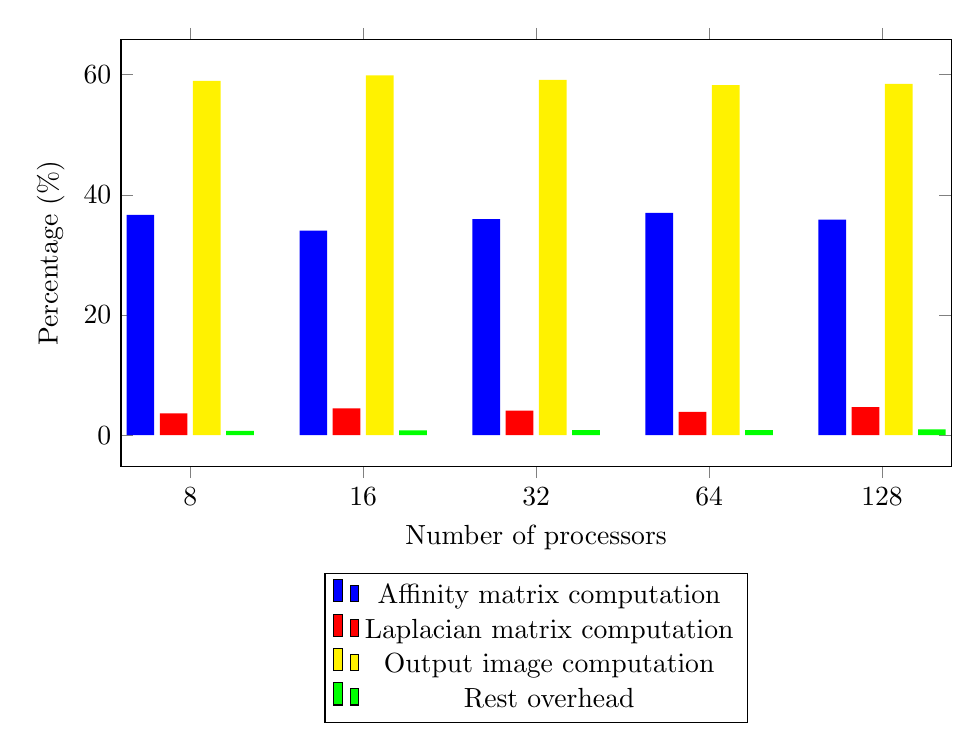
\begin{tikzpicture}
 \begin{axis}[
  ybar,
  height=7cm,
  width=\textwidth,
  xlabel=Number of processors,
  xtick={0, 1, 2, 3, 4},
  xticklabels={8, 16, 32, 64, 128},
  legend style={
   at={(0.5, -0.25)},
   anchor=north
  },
  ylabel={Percentage (\%)}]
  \addplot[draw=none, fill=blue] coordinates {
   (0, 36.67)
   (1, 34.04)
   (2, 35.96)
   (3, 37)
   (4, 35.88)};
  \addplot[draw=none, fill=red] coordinates {
   (0, 3.62)
   (1, 4.48)
   (2, 4.07)
   (3, 3.88)
   (4, 4.67)};
  \addplot[draw=none, fill=yellow] coordinates {
   (0, 58.99)
   (1, 59.9)
   (2, 59.15)
   (3, 58.26)
   (4, 58.48)};
  \addplot[draw=none, fill=green] coordinates {
   (0, 0.72)
   (1, 0.78)
   (2, 0.82)
   (3, 0.86)
   (4, 0.96)};
  \legend{
   Affinity matrix computation,
   Laplacian matrix computation,
   Output image computation,
   Rest overhead}
 \end{axis}
\end{tikzpicture}
